\FloatBarrier
\begin{figure}[!h]
\centering
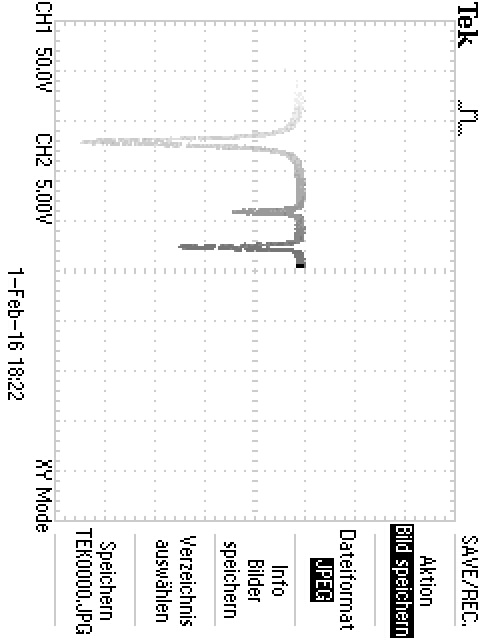
\includegraphics[scale=1,angle=90]{../Grafiken/Signalbild_RF100kHz.jpg}
\caption{Typisches Signalbild des durchgeführten Versuchs, aufgenommen bei einer Frequenz von \SI{100}{\kilo\hertz}. 
	Die Achsen sind Proportional zum anliegenden Magnetfeld ($x$) und der Transparenz des Rubidiumdampfes ($y$). 
	Zusehen sind die Minima für den Nulldurchgang des Magnetfeldes und die Resonanzstellen für die beiden 
	Rubidium-Isotope.\label{fig:signalbild_rf100khz}}
\end{figure}
\FloatBarrier